\documentclass[tikz]{standalone}
\usetikzlibrary{angles,arrows,quotes}

% Colors
\colorlet{veccol}{black!30}
% Reference frame axis styles
\tikzstyle{vec}=[-stealth,line cap=round,veccol]

\begin{document}

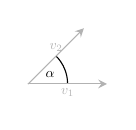
\begin{tikzpicture}[every node/.append style={scale=0.5}]
  \coordinate (O) at (0,0);
  \coordinate (A) at (1,0);
  \coordinate (B) at (45:1);
  % Vectors
  \path (A) -- (O) -- (B)
  pic ["\(\alpha\)",draw,angle radius=10mm] {angle=A--O--B};
  \draw[vec] (O) -- node [below] {\(v_{1}\)} (A);
  \draw[vec] (O) -- node [above] {\(v_{2}\)} (B);
\end{tikzpicture}

\end{document}


%%% Local Variables:
%%% mode: latex
%%% TeX-master: t
%%% End:
